\chapter{ความคืบหน้าในการพัฒนา}
\subsubsection{Backend}
ได้มีการจัดเก็บข้อมูลตลาดหุ้น และสร้างระบบอัพเดตข้อมูลแบบ real-time รายชั่วโมงไปแล้ว ได้เขียนโปรแกรมสำหรับ Fuzzy Logic ไปบางส่วนแล้ว
รวมถึงมีการลองทำตัวเว็บเซิร์ฟเวอร์ไปบ้าง โดยสามารถดู code ได้ที่ \url{https://github.com/Fuzzy-Technical-Indicator/backend}

\begin{figure}[ht]
    \centering
    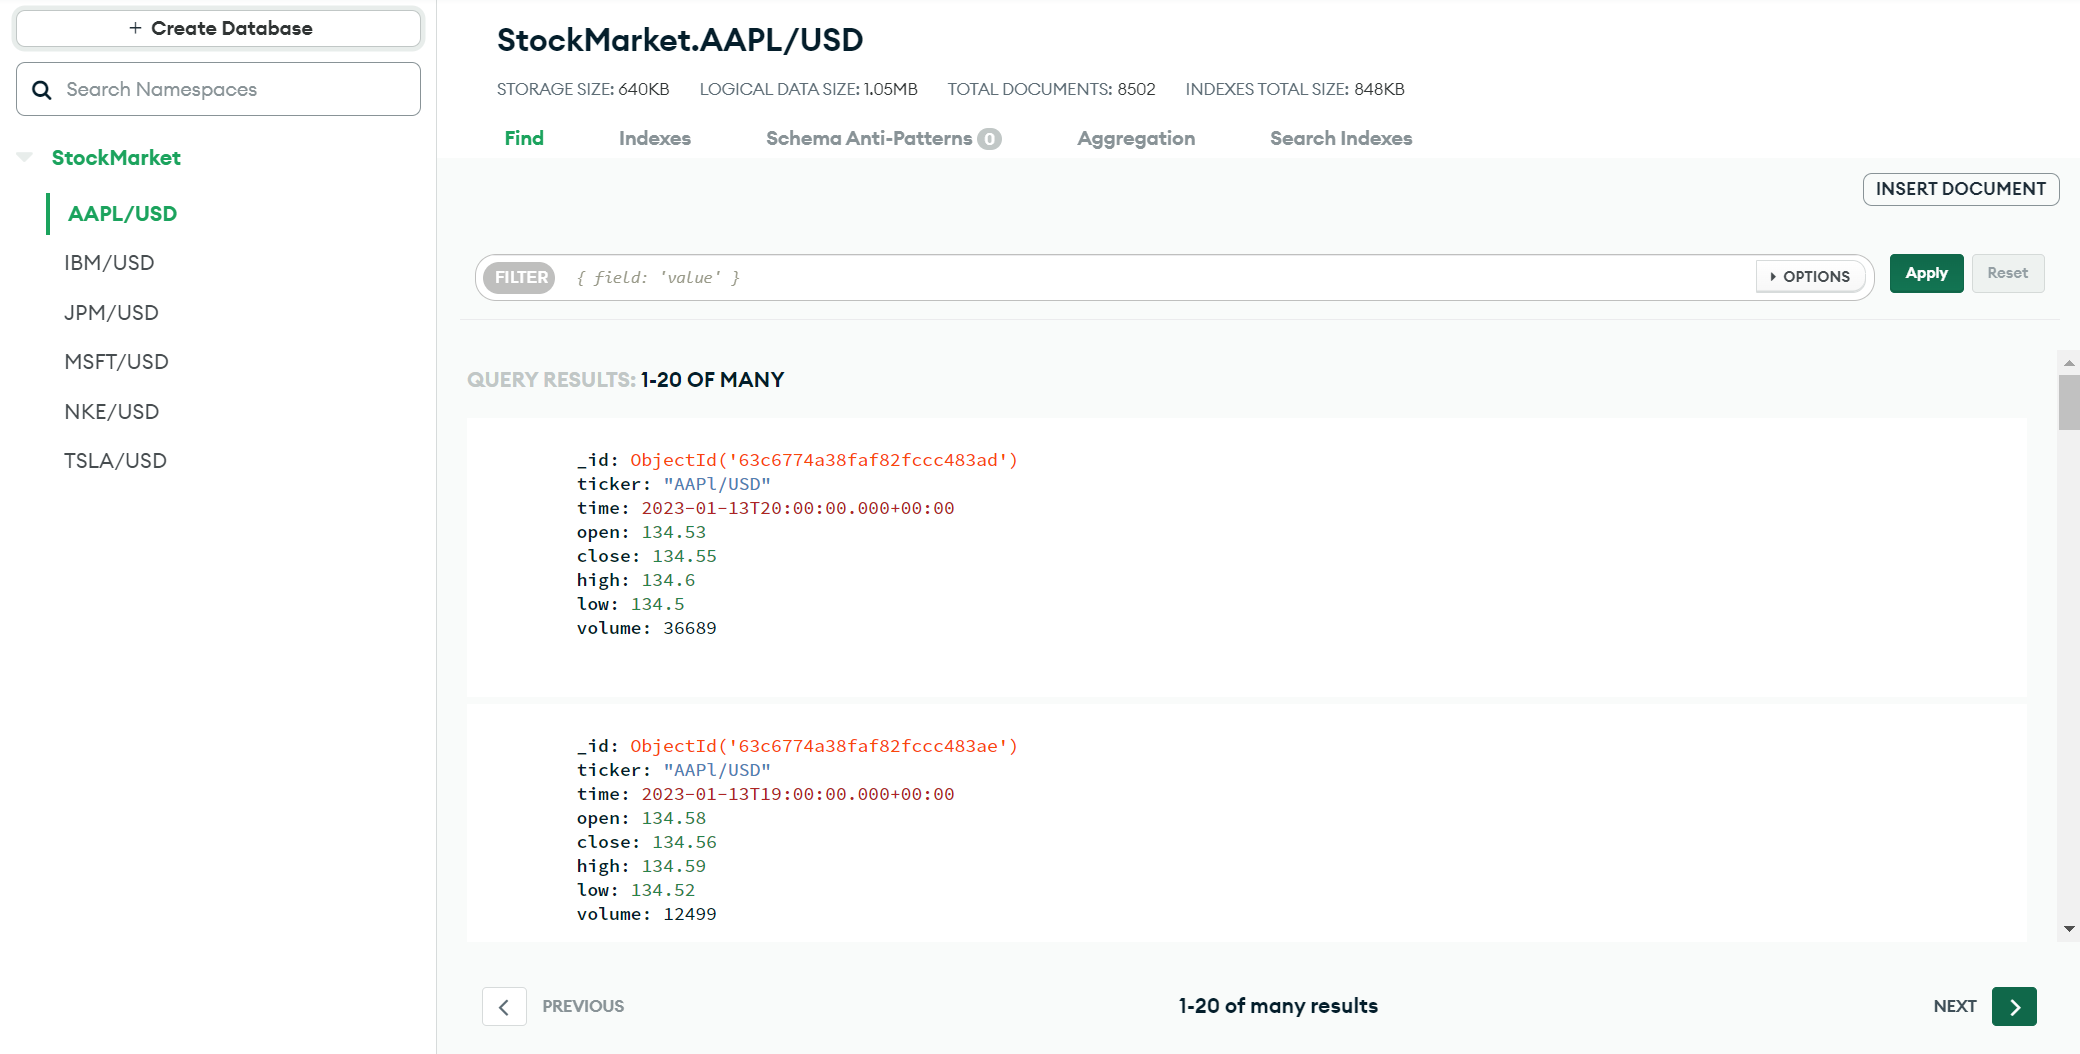
\includegraphics[width=\textwidth]{images/db_example.png}
    \caption{ตัวอย่างข้อมูลตลาดหุ้นในฐานข้อมูล}
\end{figure}
\pagebreak

\subsubsection{Frontend}
ได้มีการออกแบบหน้าตาแอปพลิเคชันทั้งแบบบนเว็บไซต์และแบบโทรศัพท์
\begin{figure}[ht]
    \centering
    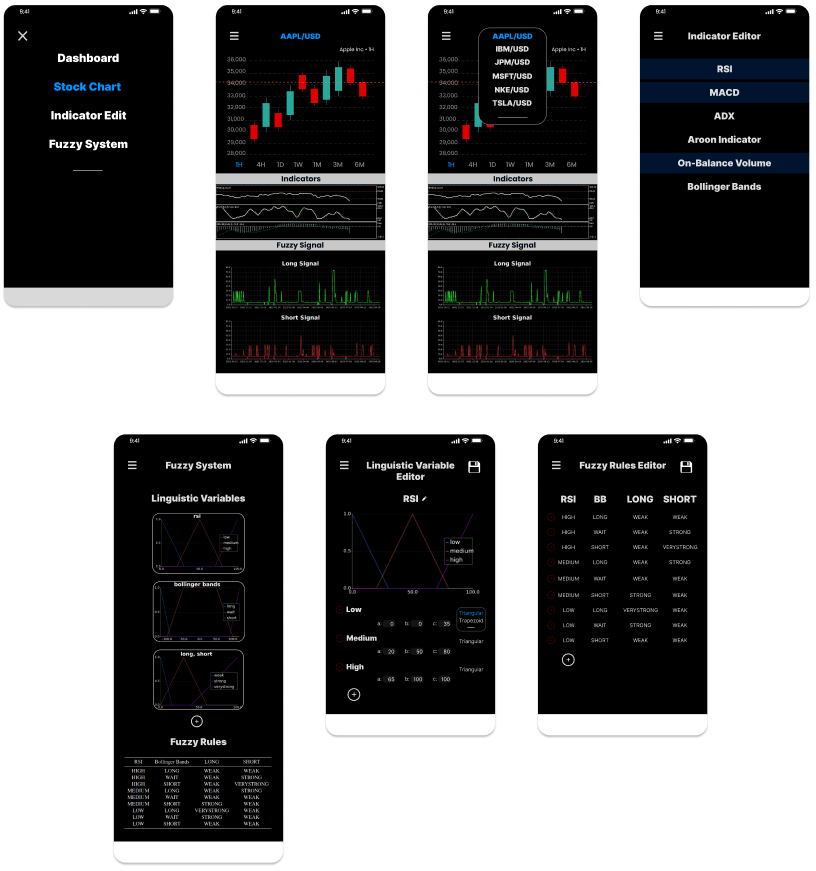
\includegraphics[width=\textwidth]{images/mobile_uiux.png}
    \caption{UI/UX ของแอปพลิเคชันบนโทรศัพท์}
\end{figure}

\begin{figure}[ht]
    \centering
    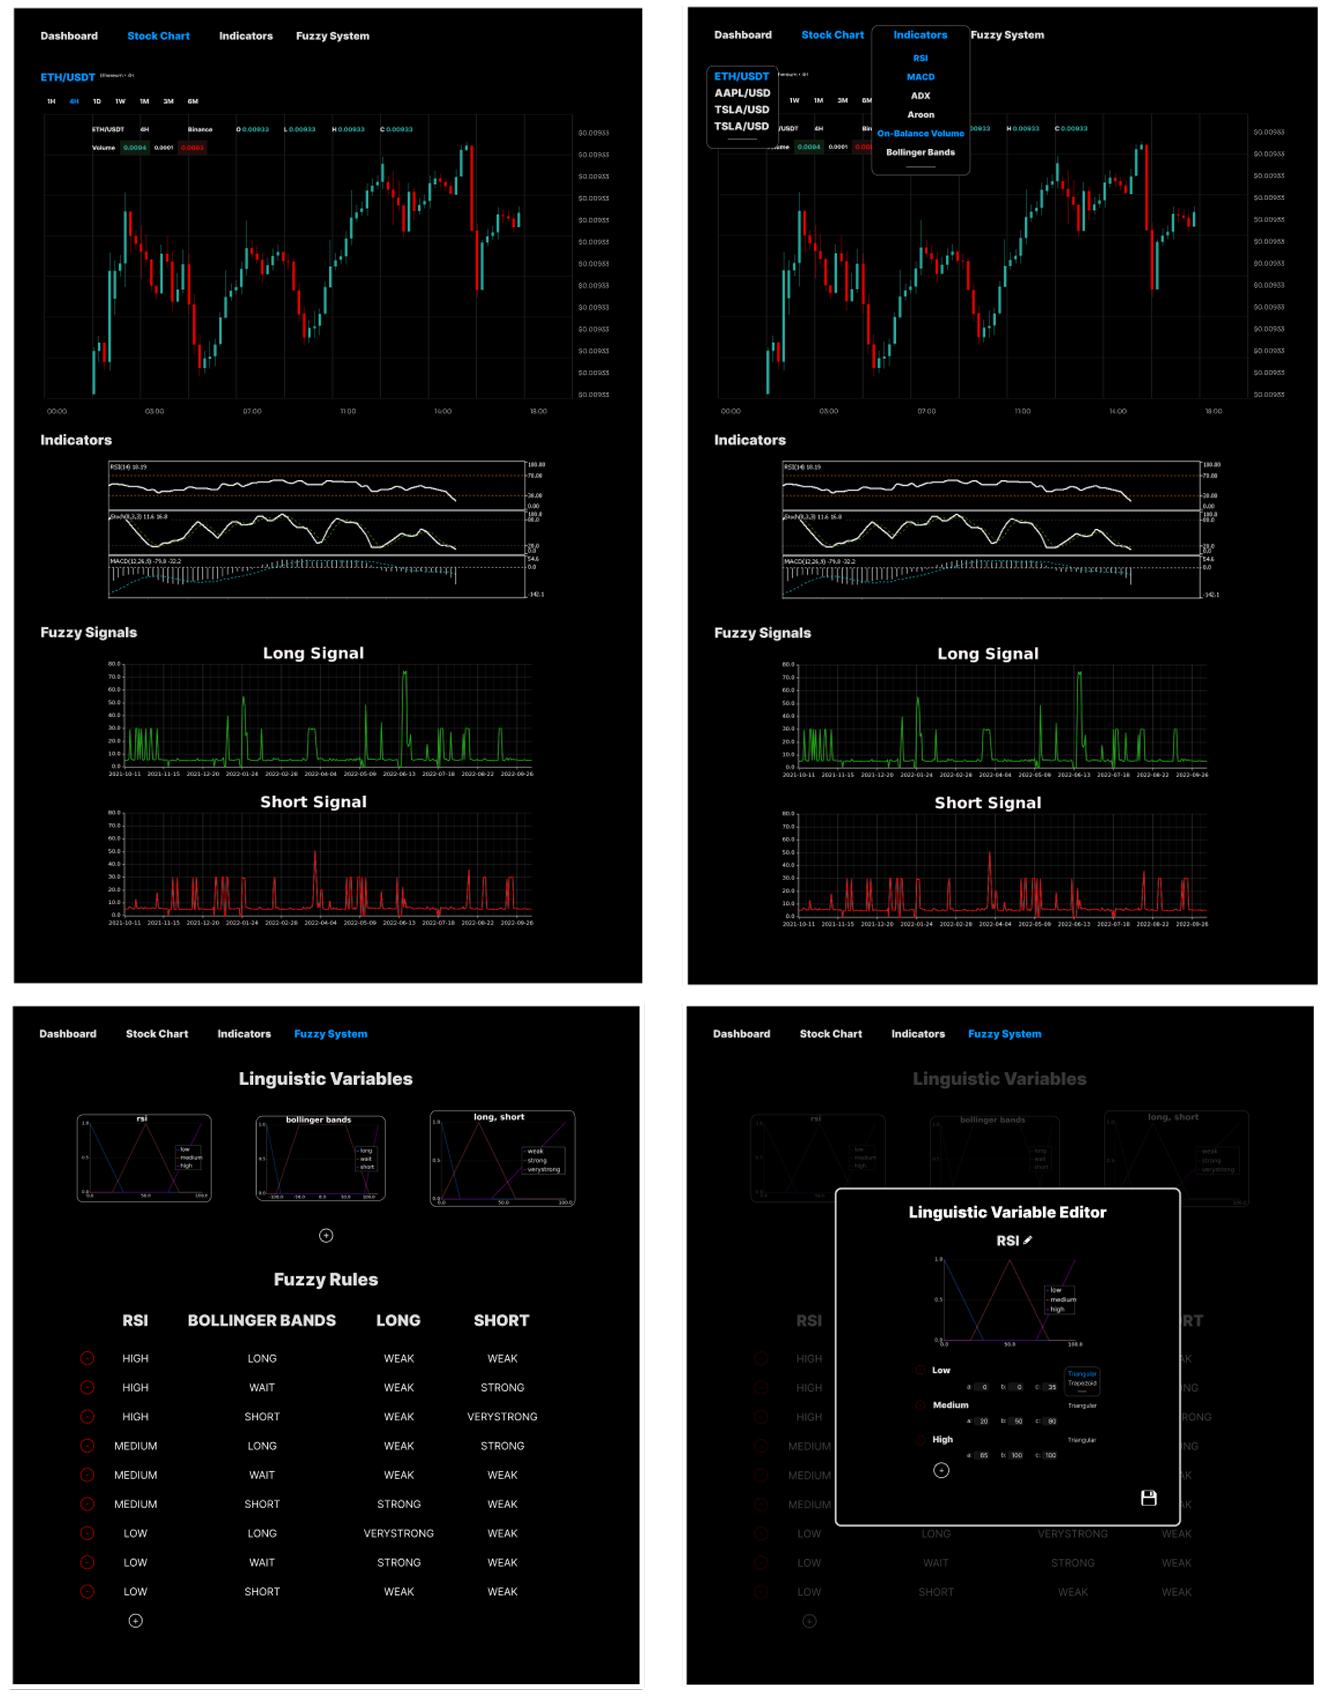
\includegraphics[width=\textwidth]{images/web_uiux.png}
    \caption{UI/UX ของเว็บไซต์}
\end{figure}

%\chapter{\ifenglish Manual\else คู่มือการใช้งานระบบ\fi}
%Manual goes here.
